%% Genatic Algorthims introduction
\begin{frame}{Genatic Algorthims}

We don't want to take just the fittest individuals, this will inhibit diversity
\end{frame}
\begin{frame}[allowframebreaks]
  \frametitle{Genetic Operations}
  \small
  Crossover operations
  \begin{itemize}
    \tiny
    \item Single point - choose a single point (two segments) to crossover
    \begin{figure}
      \centering
      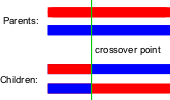
\includegraphics[width=0.2\textheight]{SinglePointCrossover.png}
    \end{figure}
    \item Two point - choose two points (three segments) to crossover
    \begin{figure}
      \centering
      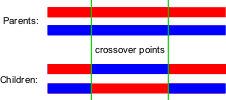
\includegraphics[width=0.2\textheight]{TwoPointCrossover.png}
    \end{figure}
    \item Uniform - Uniformly cross over based on some probablity
    \begin{figure}
      \centering
      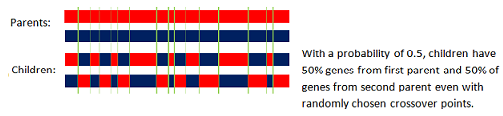
\includegraphics[width=0.2\textheight]{UniformCrossover.png}
    \end{figure}
  \end{itemize}
  \small
  Mutations
  \begin{itemize}
    \tiny
    \item Avoid local minima
  \end{itemize}
  Mutation operations
  \begin{itemize}
    \item Swap
    \item Flip - flips (inverts) all of the bits
  \end{itemize}
\end{frame}
